\documentclass{article}
\usepackage{2130,amsmath,amssymb,graphicx}
\usepackage[table]{xcolor}
\usepackage{comment}
\usepackage{amsmath}
\usepackage{listings}
\usepackage{tikz}
\usepackage{pgfplots}
\usepackage{pgfplotstable}
\usepackage{graphicx}
\usepackage{subcaption}
\usepackage{biblatex}
\addbibresource{cite.bib}
\pgfplotsset{compat=1.7}
\usetikzlibrary{shapes.geometric}
%\setlength{\arrayrulewidth}{0.5mm}
\renewcommand{\arraystretch}{1.5}

\pgfplotsset{compat=1.14,           % <-- added
            width=0.75\columnwidth,     % <-- added
            height=0.5\columnwidth % <-- added, with this the image is in aspect 4:3
            }

\title{Approximating $\pi$}
\author{Chelsea Beaton}
\date{March 2022}

\begin{document}
\maketitle

\begin{abstract}
    Since it was first discovered, $\pi$ has intrigued mathematicians and scientists alike. $\pi$ is the ratio of the circumference of a circle to the diameter of that circle. This ratio will always equal $\pi$, regardless of the size of the circle. Throughout history, many algorithms and methods have been created to try to find the exact value of $\pi$ (or as many digits as possible). Archimedes was the first person to develop an algorithm which enables the calculation of $\pi$ to any desired accuracy. This algorithm can be implemented with a computer code to generate the desired amount of digits for $\pi$. 
\end{abstract}

\section{Introduction}
% Introduce who Archimedes is and his method of estimating pi.
Archimedes was a Greek scientist born in 287 BC, who made many important discoveries and contributions to the world of science in his time. He was known to be a mathematician, physicist, astronomer, engineer, inventor and weapons-designer. \cite{arch} One of his contributions was his estimation of $\pi$, which at the time was the most precise value of $\pi$ known. Archimedes knew that $\pi$ was equal to the circumference of a circle divided by the diameter, $\pi = \frac{C}{d}$ so he used this fact to develop an algorithm which enables the calculation of $\pi$ to any desired accuracy. Archimedes started with a hexagon inscribed in a unit circle (which has a radius of $1$, and a diameter of $2$). He was able to find the side length of the hexagon, $l$, and therefore the perimeter, $P$, by multiplying $l$ by the number of sides of the inscribed polygon, $n$. He divided this value by the diameter of the circle to get his first estimation of $\pi$,
\begin{equation} \label{eq:1}
    e = \frac{P}{d} = \frac{l \cdot n}{d}
\end{equation}
Since the perimeter of an inscribed hexagon is less than the circumference of the circle it is inscribed in, he used this estimation of $\pi$ as a lower bound. Archimedes repeated this calculation with a hexagon circumscribed around a circle, and since the perimeter of this hexagon is larger than the circumference of the circle, he also had an upper bound on an estimation of $\pi$. As Archimedes increased the number of sides of the inscribed and circumscribed polygon, he was able to obtain more accurate estimations of $\pi$, since their perimeters got closer to the circumference of the circle they were bound in/around.     

\section{Method}
% Talk about how I found the side lengths of the inscribed and circumscribed hexagon. Then talk about how I found the side lengths of the inscribed and circumscribed 12-gon, so that I could proceed in an iterative fashion to find the side lengths of any n-gon. Then talk about how I can estimate a value of pi using these side lengths. 
\subsection{Finding the Side Length of Inscribed/Circumscribed Hexagons}
The first thing Archimedes had to do to implement his algorithm was find the side lengths of the inscribed and circumscribed hexagons. As seen in Figure \ref{fig:1}, the inscribed hexagon can be split into 6 equilateral triangles with angles equal to $\frac{\pi}{3}$, which can then be further split into right triangles. The hypotenuse of the right triangle touches the circle so we know that the length of it is $1$. Archimedes knew that $\sin(\frac{\pi}{6})=0.5$, so we can use this fact and the length of the hypotenuse to find the side length labeled $x$. We know that $\sin({\frac{\pi}{6}})=\frac{x}{1}$, so $x=\sin({\frac{\pi}{6}})=0.5$. This value is multiplied by $2$ to get the full side length of the hexagon, $l = 2 \cdot x = 2 \cdot 0.5 = 1$. Now we know that the side length of a hexagon inscribed within a unit circle is equal to $1$.

\begin{figure}[htp]
    \centering
    \includegraphics[width=6cm]{figure1.jpeg}
    \caption{Finding the side length of an inscribed hexagon.}
    \label{fig:1}
\end{figure}

\par In order to find the side length of the circumscribed hexagon, we need to set up a comparison between the inscribed and circumscribed hexagon. Like the inscribed hexagon, the circumscribed hexagon can be split into 6 equilateral triangles, which can then be split into 2 right triangles each. As depicted in Figure \ref{fig:2}, the hypotenuse of the smaller triangle, $r$, goes from the origin to the edge of the circle, so we know it is equal to $1$. The line that splits the equilateral triangle into 2 right triangles is also equal to $1$ because it begins at the origin and touches the edge of the circle. We need to set up a comparison between the two triangles to find the value of $y$, which corresponds to half the side length of the circumscribed hexagon. We can use half of the side length of the inscribed hexagon, $x$, the distance from the origin to the side length of the inscribed hexagon, $a$, and the distance from the origin to the side length of the circumscribed hexagon, $r$, to find a value for $y$. 
\clearpage
\begin{figure}[h]
     \centering
     \begin{subfigure}[b]{0.4\textwidth}
         \centering
         \includegraphics[width=\textwidth]{figure2.jpeg}
         \caption{Inscribed and circumscribed hexagon.}
     \end{subfigure}
     \hfill
     \begin{subfigure}[b]{0.5\textwidth}
         \centering
         \includegraphics[width=6cm]{figure3.jpeg}
         \caption{Bigger view of the triangle in Figure 2(a).}
     \end{subfigure}
     \caption{Finding the side length of an circumscribed hexagon.}
     \label{fig:2}
\end{figure}


This comparison can be written as,
\begin{equation} \label{eq:2}
    \frac{y}{r}=\frac{x}{a}.
\end{equation}
Right now, the value of $x$ is known to be $0.5$, but we need to derive an expression for $a$ in terms of $x$. The Pythagorean Theorem can be used to derive this equation, since the value of the hypotenuse of the inscribed triangle is equal to $1$, and the value of $x$ is known to be $0.5$. When deriving an expression for $a$, we obtain
\begin{equation*}
    a^2 = 1^2 - x^2
\end{equation*}
\begin{equation*}
    a = \sqrt{1-x^2}
\end{equation*}
This expression for $a$ can now be used in equation \ref{eq:2} to get this equation for $y$,
\begin{equation*}
    \frac{y}{r}=\frac{x}{a}
\end{equation*}
\begin{equation*}
    y=\frac{r \cdot x}{a}
\end{equation*}
\begin{equation*}
    y = \frac{r \cdot x}{\sqrt{1-x^2}}.
\end{equation*}
The values of all of these variables are known, so we can plug them in to obtain a value of $y$,
\begin{equation*}
    y = \frac{1 \cdot 0.5}{\sqrt{1-(0.5)^2}}
\end{equation*}
\begin{equation*}
    y=\frac{1}{2 \cdot \sqrt{0.75}}.
\end{equation*}
As we know from before, $y$ corresponds to half the side length of the circumscribed hexagon, so to get value of the full side length, $L$, we simply multiply $y$ by 2, $L = 2 \cdot y = 2 \cdot \frac{1}{2 \cdot \sqrt{0.75}} = \frac{1}{\sqrt{0.75}}$.


\subsection{Using Perimeter to Estimate $\pi$}
Now that we have obtained a value for the side lengths of the inscribed and circumscribed hexagons, we can use these values and equation \ref{eq:1} to find an estimation for $\pi$. The lower bound of our estimation of $\pi$ is equal to 
\begin{equation*}
    e = \frac{l \cdot n}{d} = \frac{1 \cdot 6}{2} = 3
\end{equation*}

\noindent and the upper bound of our estimation of $\pi$ is equal to
\begin{equation*}
    e = \frac{L \cdot n}{d} = \frac{\frac{1}{\sqrt{0.75}} \cdot 6}{2} = \frac{3}{\sqrt{0.75}} \approx 3.464.
\end{equation*}
Therefore, using Archimedes algorithm, the approximation of $\pi$ obtained when using inscribed and circumscribed hexagons is $3.0 \leq \pi \leq 3.464$.

\subsection{Finding the Side Lengths of Polygons with a Larger Number of Sides}
In order to obtain more accurate estimations for the value of $\pi$, Archimedes increased the number of side lengths of the inscribed and circumscribed n-gons so that their perimeter got closer to the value of the circumference of the circle. We can derive a formula for the side length of an inscribed dodecagon, $l_{12}$, in terms of the side length of an inscribed hexagon, $l_{6}$.
\par As seen Figure \ref{fig:3}, our goal is to find the length of $l_{12}$. Since we have previously found the value of $l_6$, if we found an expression for the side $b$, we could use the Pythagorean Theorem to find what $l_{12}$ is in terms of $l_6$.

\begin{figure}[ht]
     \centering
     \begin{subfigure}[b]{0.4\textwidth}
         \centering
         \includegraphics[width=\textwidth]{figure4.jpeg}
         \caption{Inscribed hexagon and dodecagon.}
     \end{subfigure}
     \hfill
     \begin{subfigure}[b]{0.5\textwidth}
         \centering
         \includegraphics[width=7cm]{figure5.jpeg}
         \caption{Bigger view of the triangle in Figure 3(a).}
     \end{subfigure}
     \caption{Finding the side length of an inscribed dodecagon}
     \label{fig:3}
\end{figure}


\par We know that because the line $a+b$ goes from the origin of the circle to the edge of the circle, it is equal to $1$, so $a+b=1$, or $b=1-a$. Now we can find an expression for $a$ in terms of $l_6$ by using the Pythagorean Theorem. The hypotenuse of the bigger triangle is equal to 1 since it is equal to the radius of the circle, so using the hypotenuse and half of the side of the hexagon, $\frac{l_6}{2}$, we can derive this expression for $a$,
\begin{equation*}
    1^2 = a^2 + \left( \frac{l_6}{2} \right)^2
\end{equation*}
\begin{equation*}
    1 = a^2 + \frac{(l_6)^2}{4}
\end{equation*}
\begin{equation*}
    a^2 = 1 - \frac{(l_6)^2}{4}
\end{equation*}
\begin{equation*}
    a = \sqrt{ \left( 1 - \frac{(l_6)^2}{4} \right) }
\end{equation*}

Now that we have derived an expression for $a$, we can find one for b,
\begin{equation*}
    b = 1 - a
\end{equation*}
\begin{equation*}
    b = 1 - \sqrt{1-\frac{(l_6)^2}{4}}
\end{equation*}

We can now find $l_{12}$ by using $l_6$ and our expression for $b$ in the Pythagorean Theorem,
\begin{equation*}
    (l_{12})^2 = \left( \frac{l_6}{2} \right)^2 + b^2
\end{equation*}
\begin{equation*}
    (l_{12})^2 = \frac{(l_6)^2}{4} + \left(1 - \sqrt{1-\frac{(l_6)^2}{4}}\right)^2
\end{equation*}
\begin{equation*}
    (l_{12})^2 = 2\left(1-\sqrt{1-\frac{(l_6)^2}{4}}\right)
\end{equation*}
\begin{equation*}
    l_{12} = \sqrt{2\left(1-\sqrt{1-\frac{(l_6)^2}{4}}\right)}
\end{equation*}

We have now obtained a formula to calculate the side length of a dodecagon inscribed in a circle, based on the side length of a hexagon. If we plug in the value we obtained earlier for $l_6$, we get the length of $l_{12}$ to be around $0.518$.
\par This formula that we have derived works for any number of side lengths. If we wanted to find the next side length when we double the number of sides, $l_{24}$, we simply plug the value of $l_{12}$ in our formula to obtain,
\begin{equation*}
    l_{24} = \sqrt{2\left(1-\sqrt{1-\frac{(l_{12})^2}{4}}\right)}
\end{equation*}
\begin{equation*}
    l_{24} \approx 0.261
\end{equation*}

In order to find the next lengths of the circumscribed polygons, a similar method can be implemented. 


\subsection{Implementing Archimedes Algorithm}
%How I implemented it through a computer code
Archimedes algorithm for estimating the value of $\pi$ can easily be implemented with a computer code. We want the user to be able to choose how many sides their starting n-gon has, $n_0$, and how many iterations they want their code to execute, $m$ (the number of iterations corresponds to the number of sides the final $n$-gon will have, $n_m = 2^m n_0$. The first thing the code should do is assign a proper value to the side length of the starting $n$-gon. Depending on what the user inputs for the value of $n_0$, the code will set the initial side lengths. Now the code enters a while loop which will repeat until the number of iterations executed becomes greater than the value the user input for $m$ (the number of iterations wanted). The code should now calculate and output the value of the lower and upper bounds of the estimation of $\pi$, lower\_bound = (inscribed\_side\_length * num\_sides)/2 and upper\_bound = (circumscribed\_side\_length * num\_sides)/2. Next, the side lengths of the next $n$-gon, where the number of sides are doubled, should be calculated using the method described in Section 2.3. The inscribed and circumscribed lengths are now set equal to the next side lengths, and the number of iterations is incremented.


\section{Results}
% Show a table of side lengths and estimates of pi based on those side lengths.

Table \ref{table: 1} shows the output of the computer code implementing Archimedes algorithm, starting with a hexagon and doubling the number of sides per iteration.

\begin{table}[ht]
    \centering
    \begin{tabular}{ |c|c|c|c| }
    \hline
        Iteration&Number of sides&Lower bound&Upper bound \\
        \hline
        $0$ & $6$ & $3.0$ & $3.4641016151377553$ \\
        \hline
        $1$ & $12$ & $3.1058285412302498$ & $3.2153903091734723$ \\
        \hline
        $2$ & $24$ & $3.132628613281237$ & $3.1596599420975$ \\
        \hline
        $3$ & $48$ & $3.139350203046872$ & $3.146086215131435$ \\
        \hline
        $4$ & $96$ & $3.14103195089053$ & $3.1427145996453683$ \\
        \hline
        $5$ & $192$ & $3.1414524722853443$ & $3.1418730499798233$ \\
        \hline
        $6$ & $384$ & $3.141557607911622$ & $3.141662747056848$ \\
        \hline
        $7$ & $768$ & $3.141583892148936$ & $3.141610176604689$ \\
        \hline
        $8$ & $1536$ & $3.1415904632367617$ & $3.1415970343215256$ \\
        \hline
        $9$ & $3072$ & $3.1415921060430483$ & $3.141593748771352$ \\
        \hline
        $10$ & $6144$ & $3.1415925165881546$ & $3.141592927385097$ \\
        \hline
    \end{tabular}
    \caption{Lower and upper bounds of the estimation of $\pi$ starting with a hexagon and doubling the number of sides for each iteration.}
    \label{table: 1}
\end{table}
\clearpage
Table \ref{table: 2} shows the output of the computer code implementing Archimedes algorithm, starting with a pentagon and doubling the number of sides per iteration.

\begin{table}[ht]
    \centering
    \begin{tabular}{ |c|c|c|c| }
    \hline
        Iteration&Number of sides&Lower bound&Upper bound \\
        \hline
        $0$ & $5$ & $2.938926261462366$ & $3.6327126400268046$ \\
        \hline
        $1$ & $10$ & $3.090169943749474$ & $3.249196962329063$ \\
        \hline
        $2$ & $20$ & $3.1286893008046186$ & $3.1676888064907254$ \\
        \hline
        $3$ & $40$ & $3.1383638291137923$ & $3.1480682729847373$ \\
        \hline
        $4$ & $80$ & $3.1407852607254947$ & $3.143208560613571$ \\
        \hline
        $5$ & $160$ & $3.141390793700371$ & $3.141996443420316$ \\
        \hline
        $6$ & $320$ & $3.141542187887282$ & $3.141693589371422$ \\
        \hline
        $7$ & $640$ & $3.1415800371154248$ & $3.1416178868055566$ \\
        \hline
        $8$ & $1280$ & $3.1415894994663325$ & $3.1415989618481333$ \\
        \hline
        $9$ & $2560$ & $3.1415918650251795$ & $3.141594230651528$ \\
        \hline
        $10$ & $5120$ & $3.141592456418232$ & $3.1415930478550487$ \\
        \hline
    \end{tabular}
    \caption{Lower and upper bounds of the estimation of $\pi$ starting with a pentagon and doubling the number of sides for each iteration.}
    \label{table: 2}
\end{table}

\section{Analysis}
% Compare the estimations of pi using 3-gons, 4-gons, 5-gons and 6-gons to see which one will converge to an acceptable estimation of pi the fastest (maybe include graphs for this, plot the difference and see which one goes to 0 first). Also verify historical estimations of pi.
\subsection{Rate of Convergence}
Our code has been developed to accept triangles, squares, pentagons and hexagons as starting $n$-gons. Each of these $n$-gons will converge to $\pi$ at a different rate. Figure \ref{graph:1} shows the difference between the high and low estimation of $\pi$ at each iteration for each n-gon we used.
\par As shown in Figure \ref{graph:1}, eventually the high and low estimates for each $n$-gon become so close together that they seem to reach a difference of $0$. However, the $n$-gon that produces the high and low estimates that are closest together (produces the smallest difference), is the hexagon. This tells us that using hexagons as our starting $n$-gon will produce an acceptable accuracy of $\pi$ the fastest. \clearpage
\begin{figure}[ht]
\begin{center}

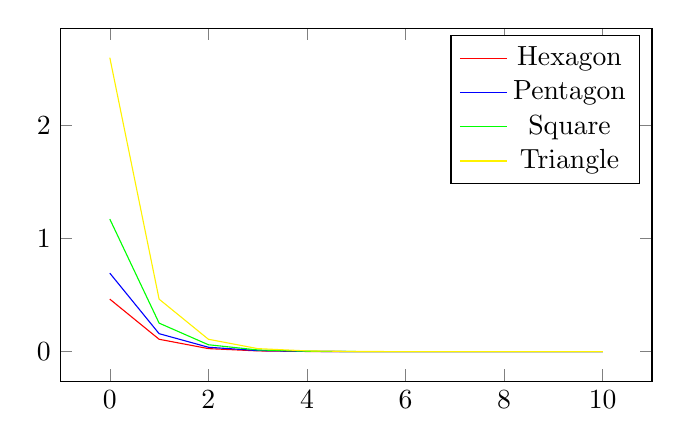
\begin{tikzpicture}
\begin{axis}
    xlabel = Iteration,
    ylabel = Difference,
    legend style = {at={(0.0,.91)},anchor=west}
    ]
\addplot[color=red] coordinates {
    (0, 0.4641016151377553)
    (1, 0.10956176794322259)
    (2, 0.027031328816263134)
    (3, 0.006736012084562759)
    (4, 0.0016826487548384783)
    (5, 0.0004205776944790074)
    (6, 0.00010513914522602974)
    (7, 2.6284455753255997e-05)
    (8, 6.571084763873358e-06)
    (9, 1.6427283036080098e-06)
    (10,  4.1079694224066543e-07)
};

\addplot[color=blue] coordinates {
    (0, 0.6937863785644387)
    (1, 0.159027018579589)
    (2, 0.03899950568610677)
    (3, 0.009704443870945045)
    (4, 0.0024232998880764356)
    (5, 0.0006056497199447008)
    (6, 0.0001514014841399458)
    (7, 3.784969013187478e-05)
    (8, 9.4623818007733e-06)
    (9, 2.365626348588279e-06)
    (10,  5.914368168546957e-07)
};

\addplot[color=green] coordinates {
    (0, 1.1715728752538102)
    (1, 0.25224104006404247)
    (2, 0.06115272581647524)
    (3, 0.01517641688331528)
    (4, 0.003787228291165068)
    (5, 0.0009463790096999602)
    (6, 0.0002365680248210822)
    (7, 5.914033529919038e-05)
    (8, 1.4784976848147835e-05)
    (9, 3.696244953665939e-06)
    (10, 9.240182303749123e-07)
};

\addplot[color=yellow] coordinates {
    (0, 2.598076211353316)
    (1, 0.46410161513775483)
    (2, 0.10956176794322259)
    (3, 0.027031328816263134)
    (4, 0.006736012084562759)
    (5, 0.0016826487548384783)
    (6, 0.0004205776944790074)
    (7, 0.00010513914522602974)
    (8, 2.6284455753255997e-05)
    (9, 6.571084763873358e-06)
    (10, 1.6427283036080098e-06)
};

\legend{Hexagon, Pentagon, Square, Triangle}
\end{axis}
\end{tikzpicture}
\end{center}
\caption{Comparison of the margin of error between the high and low estimates of $\pi$ for starting $n$-gons.}
\label{graph:1}
\end{figure}

\subsection{Historical Estimations of $\pi$}
The earliest written estimation of $\pi$ was from the ancient Babylonians between 1900 - 1680BC. It is not clear how the Babylonians found their approximation of $\pi$, but it has been recorded that they found that $\pi$ was equal to $\frac{25}{8}$. \cite{david}
\par Another early estimation of $\pi$ can be found in the Bible. The biblical verse quoted (1 Kings 7:23) says: `measuring 10 cubits from rim to rim It took a line of 30 cubits to measure around it'. It also says `It was a handbreadth in thickness'. A cubit is an ancient measure of length, approximately equal to the length of a forearm, or about 18 inches. A handbreadth is also an ancient measure of length, approximately the breadth of a hand, or about 3 inches. Using these units of measurement, we can approximate the inner diameter of the bowl to be 174 inches and the inner circumference would be 540 inches, which gives $\frac{540}{170}$ or $3.10$ as an approximation of $\pi$. \cite{kevin}
\par In 264 CE, Chinese mathematician Liu Hui independently developed the same algorithm as Archimedes. He estimated $\pi = 3.14159$ using a $3072$-gon. We can verify Liu Hui's estimation using the we code wrote. As seen in Table \ref{table: 1}, using a 3072-gon, the lower bound of the estimation of $\pi$ is $3.1415921060430483$ and the upper bound is $3.141593748771352$. Both of these bounds round to $3.14159$, so we can say that Liu Hui was accurate with his estimation.
\par The first person to decribe $\pi$ using an infinite product was François Viète in the end of the 16th century. \cite{david} Viète described $\pi$ with the formula, $\frac{2}{\pi} = \frac{\sqrt{2}}{2} \cdot \frac{\sqrt{2+\sqrt{2}}}{2} \cdot \frac{\sqrt{2 + \sqrt{2+\sqrt{2}}}}{2}...$. Viètes formula was not very useful in actually calculating a value for $\pi$ because it took too many iterations to converge, but it was a very significant discovery in mathematics because it was the first instance of an infinite product.

\section{Conclusion}
Throughout history, significant improvements have been made when it comes to estimating digits for $\pi$. Right now, it is estimated that there are around 62.8 trillion digits of $\pi$ known. The reason mathematicians and scientists want to find as many digits of $\pi$ as possible is $\pi$ is often used in the `development and testing of supercomputers and new high-precision multiplication algorithms'. \cite{convo} The more digits of $\pi$ we have, the more accurate these algorithms can be. The second reason for researching $\pi$ is simply because we still don't know much about it. Although the existence of $\pi$ was discovered centuries ago, there are still fundamental unanswered questions about the way its digits behave. Algorithms discovered by people like Archimedes, Liu Hui and François Viète paved the way for modern day mathematicians, and are so fundamental that they are still being studied today. 


\printbibliography
\end{document}
